\documentclass[12pt,a4paper]{article}
\usepackage[OT1]{fontenc}
\usepackage{amsmath}
\usepackage{amsfonts}
\usepackage{amssymb}
\usepackage{graphicx}
\usepackage{array}
\usepackage{cancel}
\usepackage{caption}
\usepackage{wrapfig}
\usepackage{secdot}
\usepackage{indentfirst}
\usepackage[left=1.5cm,right=1.5cm,top=0.3cm,bottom=1.5cm,includefoot,footskip=1.5cm]{geometry}
\usepackage[utf8]{inputenc}
\usepackage[english, russian]{babel}
\DeclareMathOperator{\sinc}{sinc}
\begin{document}
\textbf{
\begin{flushright}
Илья Кочергин, 626 группа
\end{flushright}}
\paragraph{\large Работа 3.6.1}
\paragraph{\Large Спектральный анализ электрических сигналов}
\paragraph{Цель работы:}изучение спектрального состава периодических электрических сигналов
\paragraph{Оборудование:}персональный компьютер, USB-осциллограф АКИП-4107, функциональный генератор WaveStation 2012, соединительные кабели.
\section{Теоретическая справка}
\paragraph{Ряд Фурье.} Пусть имеется периодическая функция $f(t)$ с периодом $T$. Из курса математического анализа за следующий семестр известно (пока еще нет, но будет), что ее можно разложить в бесконечную сумму гармонических функций:
\begin{equation}
f(t) = \frac{a_0}{2} + \sum\limits_{n=1}^{\infty}[a_n\cos(n\omega t) + b_n\sin(n\omega t)],
\end{equation}
где $\omega = \frac{2\pi}{T}$~--- частота сигнала, а коэффициенты $a_n$ и $b_n$ определяются формулами:
\begin{gather}
a_n = \int\limits_{t_1}^{t_1+T}f(t)\cos(n\Omega t)dt;\\
b_n = \int\limits_{t_1}^{t_1+T}f(t)\sin(n\Omega t)dt,
\end{gather}
при этом начальный предел интегрирования $t_1$ можно выбрать произвольно. 

\noindent \emph{Амплитудной спектральной функцией} $F(\omega)$ называется зависимость амплитуды гармоник от их частоты, из (1) амплитуда n-й гармоники $A_n$ выражается формулой
\begin{equation}
A_n = \sqrt{a_n^2 + b_n^2}.
\end{equation}
Для периодической функции $F(\omega)$ выражается очевидным образом:
\begin{equation}
\begin{cases}
F(\omega) = A_n,&\text{если}~\omega = k\Omega~(k\text{~--- натуральное число или 0});\\
F(\omega) = 0,&\text{иначе}.\\
\end{cases}
\end{equation}
\paragraph{Периодические прямоугольные импульсы.} Рассмотрим последовательность прямоугольных импульсов с амплитудой $V_0$, длительностью $\tau$ и периодом повторения $T$. Будем также считать, что она симметрична относительно $t=0$. Определим среднее значение амплитуды из формул (1-3):
\begin{equation}
\langle V\rangle = \frac{a_0}{2} = \frac{1}{T}\int\limits_{0}^{T}V(t)dt = V_0\frac{\tau}{T} = V_0\tau f,
\end{equation}
где $f = \frac{1}{T}$~--- частота сигнала. Аналогично определяются амплитуды косинусных составляющих (т.к. $V(t)$~--- четная функция, то все синусные амплитуды нулевые):
\begin{equation}
a_n = 2V_0\tau f\sinc \frac{n\Omega\tau}{2} =2V_0\tau f\sinc(n\pi f\tau).
\end{equation}
\emph{Шириной спектра} $\Delta\omega$ будем называть первую циклическую частоту $\omega$ (кратную $\Omega)$, при которой $F(\omega)$ обращается в ноль. Очевидно, что данное определение корректно при $\frac{T}{\tau} = z$, где $z$~--- натуральное число. Тогда из (7) следует выражение
\begin{equation}
\Delta\omega = \frac{2\pi}{\tau},
\end{equation}
что можно переписать в виде выражения
\begin{equation}
\Delta\omega\tau = 2\pi,
\end{equation}
называемое \emph{соотношением неопределенности}. Если ввести частотную ширину $\Delta\nu = \frac{\Delta\omega}{2\pi}$, то оно примет вид
\begin{equation}
\Delta\nu\tau = 1.
\end{equation}
\paragraph{Периодическая последовательность цугов.} Теперь рассмотрим последовательность цугов гармонического колебания $V_0\cos(\omega_0 t)$ с длительностью цуга $\tau$ и периодом повторения $T$. Функция $f(t)$ снова является четной, поэтому $b_n = 0$. Коэффициенты $a_n$ выражаются формулой
\begin{equation}
a_n = V_0\tau f(\sinc[\pi\tau(f_0 - nf)] + \sinc[\pi\tau(f_0 + nf)]),
\end{equation}
где $f_0 = \frac{\omega_0}{2\pi}$~--- частота цуга. Для простоты рассмотрим случай, когда в цуге целое число полных колебаний ($f\tau = \pi k$), и, кроме того, $\frac{T}{\tau} = z$ ($k$ и $z$~--- натуральные числа). Тогда спектральная ширина также выражается по формуле (8), при этом максимум $F(\omega)$ достигается при $\omega = \omega_0$.
\paragraph{Модулированные колебания} Рассмотрим колебания, амплитуда которых медленно меняется по гармоническому закону:
\begin{equation}
A(t) = A_0(1+m\cos(\Omega t))\cos(\omega_0 t).
\end{equation}
Величина $m$ называется коэффициентом модуляции. Его можно найти по формуле
\begin{equation}
m = \frac{A_{max} - A_{min}}{A_{max} + A_{min}},
\end{equation}
где $A_{max}$ и $A_{min}$~--- минимальная и максимальная амплитуды соответственно. Спектральное разложение тривиально:
\begin{equation}
A(t) = A_0\cos(\omega_0 t) + \frac{A_0 m}{2}\cos((\omega_0 + \Omega)t) + \frac{A_0 m}{2}\cos((\omega_0 - \Omega)t).
\end{equation}
Таким образом, спектр содержит 3 составляющих. Основная компонента представляет собой исходное немодулированное колебание с несущей частотой $\omega_0$ и амплитудой $A_\text{осн}=A_0$~--- первое слагаемое в правой части; боковые компоненты спектра соответствуют гармоническим колебаниям с частотами $(\omega_0+\Omega)$ и $(\omega_0-\Omega)$~--- второе и третье слагаемые. Амплитуды этих двух колебаний одинаковы и составляют $\frac{m}{2}$ от амплитуды немодулированного колебания: $A_\text{бок} = A_0\frac{m}{2}$.
\newpage
\section{Измерение спектра прямоугольных импульсов}
\begin{wrapfigure}{r}{0.45\textwidth}
\centering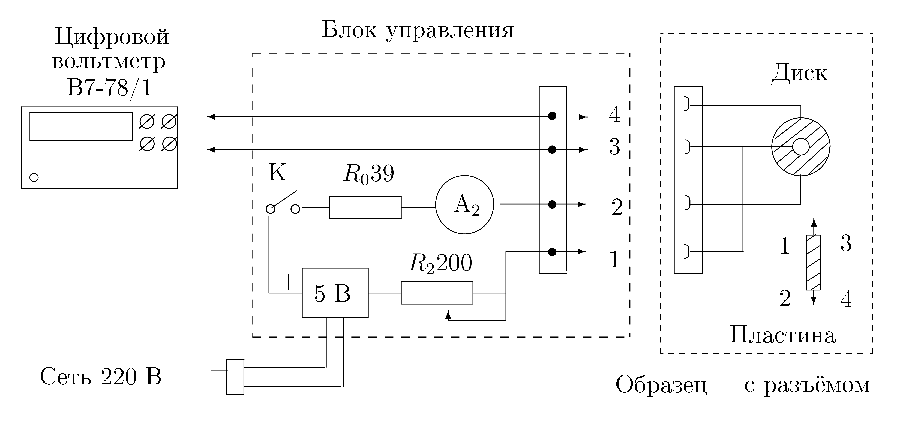
\includegraphics[width = 0.45\textwidth]{Pct1}
\captionsetup{justification = centering}
\caption{Схема установки \label{Pct1}}
\end{wrapfigure}
\paragraph{Экспериментальная установка.} Схема установки представлена на рис.1. С помощью функционального генератора можно получать до двух сигналов различной формы, которые подаются на каналы осциллографа. Можно также рассматривать их в режиме спектрометра. Эта установка общая для всех последующих частей.

Будем исследовать спектр прямоугольных импульсов амплитудой 1 В. Сначала рассмотрим, как меняется спектр при увеличении $\tau$ вдвое при неизменной частоте, и при увеличении частоты вдвое при неизменном $\tau$. Далее снимем данные для воспроизведения спектров, а также построения графика $\Delta\nu(\tau)$ для проверки соотношения неопределенностей.
\paragraph{Обработка результатов.} При увеличении $\tau$ вдвое спектральная ширина уменьшается в 2 раза, расстояние между пиками не изменяется, а амплитуда становится равной удвоенной амплитуде пика, соответствующего удвоенной частоте. При увеличении $f$ вдвое расстояние между пиками также увеличивается вдвое, спектральная ширина неизменна, а амплитуда становится равной удвоенной амплитуде пика с той же частотой.

Данные для построения спектров не заслуживают занесения в отдельную таблицу, ибо нет необходимости в их пересчете (еще их слишком много), поэтому они представлены графически (рис. 2), при этом их пришлось отнормировать. На этих графиках также проведены теоретические зависимости (7), при этом амплитуды берутся по модулю в силу (4). Частоты одинаковы и равны 1 кГц.
\begin{figure}[h!]
\centering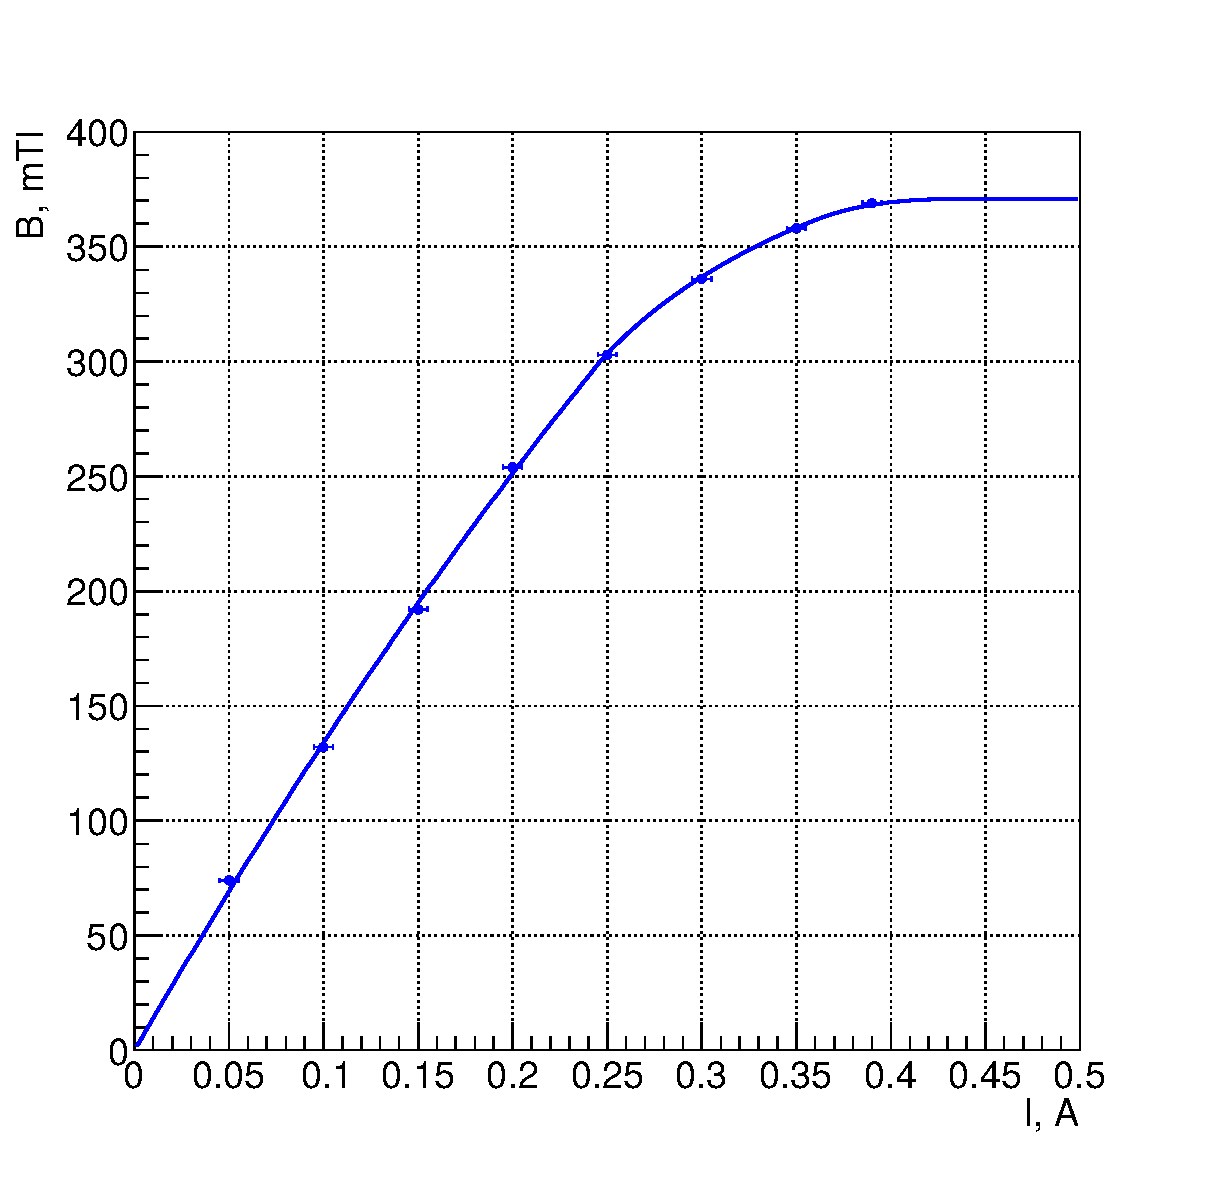
\includegraphics[width = 0.99\textwidth]{Plot1}
\captionsetup{justification = centering}
\caption{Спектры прямоугольных импульсов, слева $\tau = 50~\text{мкс}$, справа 100 мкс. \label{Pct1}}
\end{figure}
Данные для построения графика $\Delta \nu(\tau)$ представлены в таблице 1.
\newpage
\begin{table}\centering
\begin{tabular}[ht]{|*{10}{c|}}
\hline
$\tau,~\text{мс}$&40&60&80&100&120&140&160&180&200\\
\hline
$\Delta \nu,~\text{Кгц}$&24.2&16.2&12.0&9.9&8.4&7.1&6.3&5.5&5.0\\
\hline
$\frac{1}{\tau},~\text{кГц}$&25.0&16.7&12.5&10.0&8.3&7.1&6.3&5.6&5.0\\
\hline
\end{tabular}
\caption{Данные для графика $\Delta \nu(\tau)$}
\end{table}
\begin{wrapfigure}{r}{0.45\textwidth}
\centering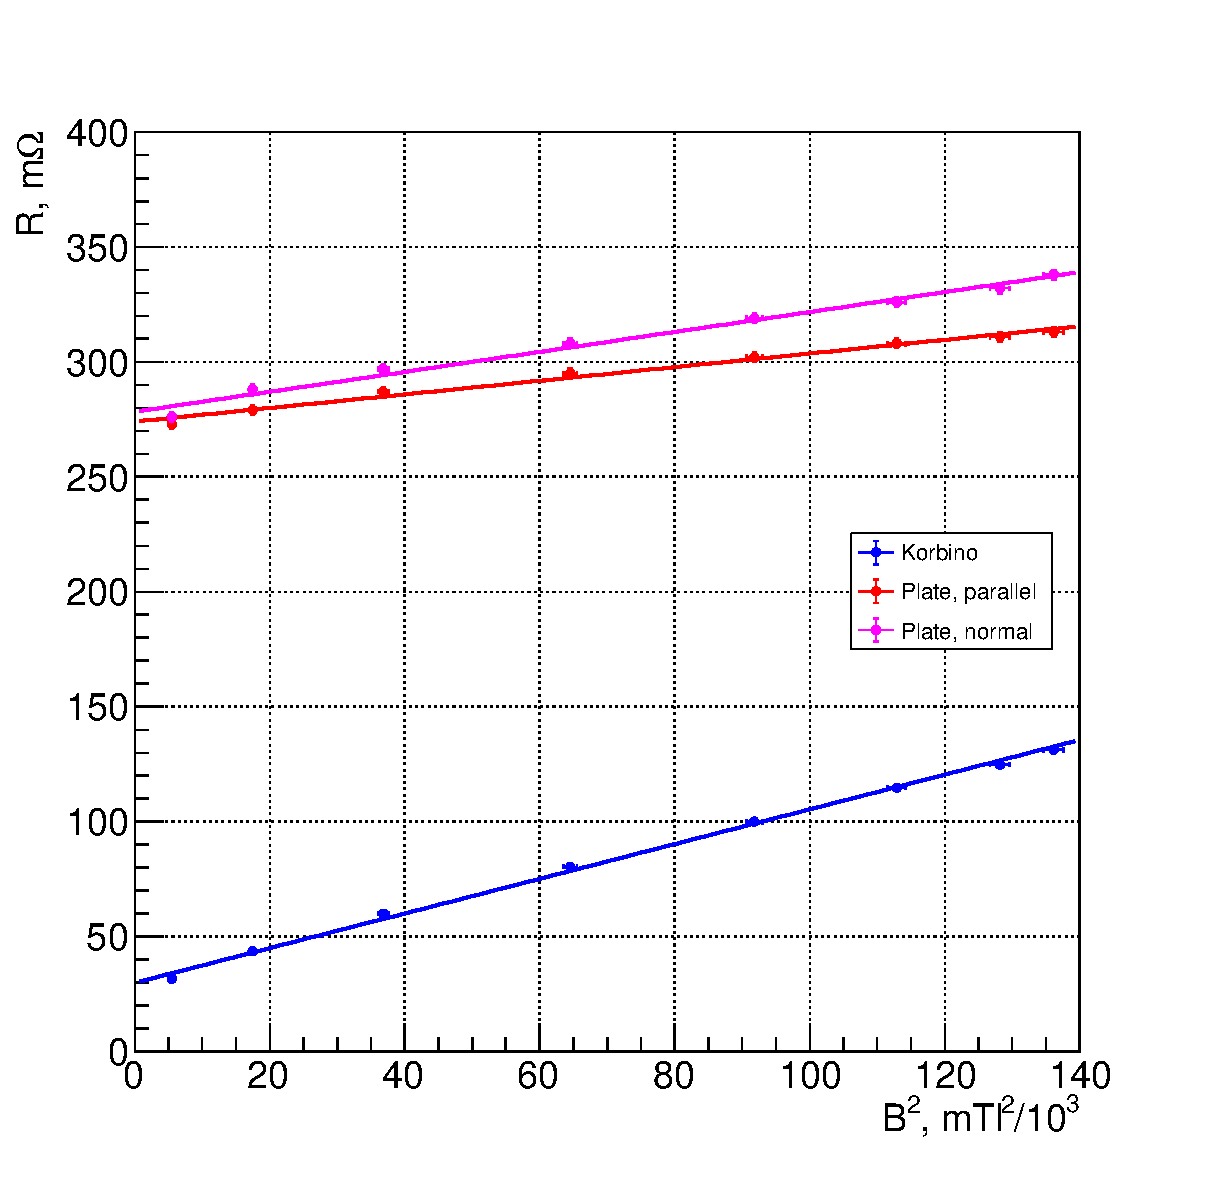
\includegraphics[width = 0.45\textwidth]{Plot2}
\captionsetup{justification = centering}
\caption{График $\Delta \nu(\tau)$ \label{Plot2}}
\vspace{-60pt}
\end{wrapfigure}
График представлен на рис. 3, его коэффициент наклона равен $1.03\pm0.01$, что близко к 1 и подтверждает соотношение неопределенностей. Погрешность $\tau$ считалось нулевой, погрешность $\Delta \nu$~--- 0.2 кГц.
\section{Измерение спектра последовательности цугов}
\paragraph{Экспериментальная установка.} Установка та же, для создания цугов перемножается синусоидальный и прямоугольно-импульсный сигналы.

Будем исследовать спектр последовательности цугов с амплитудой 1 В$^2$. Проследим, как он меняется при изменении $\tau$ и несущей частоты, и снимем зависимость расстояния между пиками $\delta\nu$ ($f$), она должна быть линейной с коэффициентом наклона 1 и свободным членом 0. Кроме того, снимем 2 спектральные картины.
\paragraph{Обработка данных.} При увеличении $\tau$ вдвое спектральная ширина уменьшается в 2 раза, расстояние между пиками не изменяется, а амплитуда высшего пика увеличивается в 2 раза. При изменении несущей частоты происходит сдвиг картины (ее центр соответствует этой частоте). Спектры для $f_0 = 30$ кГц и $\tau = 100$ мкс представлены на рис. 4 вместе с теоретическими кривыми (экспериментальные точки опять пришлось отнормировать).
\begin{figure}[h!]
\centering\includegraphics[width = 0.99\textwidth]{Plot3}
\captionsetup{justification = centering}
\caption{Спектры последовательности цугов, слева $f = 1~\text{кГц}$, справа 2 кГц. \label{Plot3}} 
\end{figure}

Данные для построения $\delta\nu(f)$ представлены в таблице 2, погрешность $\delta\nu$ считаем равной $0.01~\text{кГц}$ ($f$ считаем известной точно).

\begin{table}\centering
\begin{tabular}[ht]{|*{6}{c|}}
\hline
$f,~\text{кГц}$&0.50&1.00&2.00&4.00&5.00\\
\hline
$\Delta \nu,~ Кгц$&0.50&1.01&2.00&4.00&5.00\\
\hline
\end{tabular}
\caption{Данные для графика $\delta\nu(f)$}
\end{table}
\begin{wrapfigure}{r}{0.45\textwidth}
\centering\includegraphics[width = 0.45\textwidth]{Plot4}
\captionsetup{justification = centering}
\caption{График $\delta\nu(f))$ \label{Plot4}}
\vspace{-60pt}
\end{wrapfigure}
График представлен на рис. 4, его коэффициент наклона равен $1.000\pm0.001$, что близко к 1 и подтверждает теорию.
\section{Измерения спектра модулированных колебаний}
\paragraph{Схема установки.} Для получения модулированных по амплитуде колебаний будем использовать перемножение двух синусоидальных сигналов.

Будем исследовать спектр модулированных по амплитуде колебаний с несущей частотой 25 кГц и модулирующей частотой 1 кГц (этот сигнал сдвинут относительно 0). Меняя двойную амплитуду канала с несущей частотой, получим зависимость $\frac{A_\text{бок}}{A_\text{осн}}(m)$, она должна быть прямой пропорциональностью с коэффициентом 0.5. Кроме того, посмотрим, как меняется картина при изменении $\tau$ при 100\% глубине модуляции.
\paragraph{Обработка данных} Все необходимые данные представлены в таблице 3.
\begin{table}[h!]\centering
\begin{tabular}[ht]{|*{8}{c|}}
\hline
$2U_\text{мод}, \text{В}$&0.2&0.5&0.8&1.1&1.4&1.7&2.0\\
\hline
$2A_\text{max},~\text{В}^2$&1.11&1.25&1.39&1.55&1.69&1.84&1.93\\
\hline
$2A_\text{min},~\text{В}^2$&0.90&0.74&0.62&0.46&0.32&0.16&0.00\\
\hline
$A_\text{осн},~\text{В}^2$&0.66&0.66&0.66&0.66&0.66&0.66&0.66\\
\hline
$A_\text{бок},~\text{В}^2$&0.03&0.08&0.13&0.18&0.23&0.29&0.33\\
\hline
$m$&0.10&0.25&0.39&0.54&0.68&0.84&1.00\\
\hline
$\frac{A_\text{бок}}{A_\text{осн}}$&0.05&0.12&0.20&0.27&0.35&0.44&0.50\\
\hline
$\Delta m$&0.02&0.02&0.02&0.02&0.02&0.02&0.02\\
\hline
$\Delta\frac{A_\text{бок}}{A_\text{осн}}$&0.02&0.02&0.02&0.02&0.02&0.02&0.02\\
\hline
\end{tabular}
\caption{Данные для графика $\frac{A_\text{бок}}{A_\text{осн}}(m)$}
\end{table}
Очевидно, что~для~удвоенных амплитуд формула (13) останется справедливой. Значком $\Delta$ здесь обозначены погрешности, вычисленные по известным формулам для погрешностей измеряемых амплитуд 0.01 В$^2$.
\newpage
\begin{wrapfigure}{r}{0.45\textwidth}
\centering\includegraphics[width = 0.45\textwidth]{Plot5}
\captionsetup{justification = centering}
\caption{График $\delta\nu(f))$ \label{Plot5}}
\vspace{-60pt}
\end{wrapfigure}

График зависимости $\frac{A_\text{бок}}{A_\text{осн}}(m)$ представлен на рис. 5. Его коэффициент наклона равен $0.51\pm0.01$, что близко к теоретическому значению. Полная модуляция происходит при $2U_\text{мод}$ = 2.0 В, при увеличении $\tau$ в два раза расстояние между боковыми пиками увеличивается в 2 раза, при этом основной пик остается на месте и амплитуды не меняются.
\section{Вывод.} Работа выполнена, все необходимые величины измерены. И, хотя есть несовпадения с теорией, качественные картины удовлетворяют ожиданиям.
\end{document}